\documentclass{article}%
\usepackage[T1]{fontenc}%
\usepackage[utf8]{inputenc}%
\usepackage{lmodern}%
\usepackage{textcomp}%
\usepackage{lastpage}%
\usepackage{authblk}%
\usepackage{graphicx}%
%
\title{Preparation of Monoclonal Antibodies Cross{-}Reactive with Orthopoxviruses and Their Application for Direct Immunofluorescence Test}%
\author{Matthew Howard}%
\affil{Department of Genetics, Washington University School of Medicine, St. Louis, Missouri, United States of America}%
\date{01{-}01{-}2012}%
%
\begin{document}%
\normalsize%
\maketitle%
\section{Abstract}%
\label{sec:Abstract}%
The role of BMP{-}9 protein in BMP3{-}positive human osteosarcoma cell proliferation and migration is well known. More recently, researchers have discovered a positive interaction between BMP{-}9 and PI3K/AKT{-}active pancreatic cancer cell receptors (PCCRs) and showed that this interaction has positive effects on epithelial progenitor cells (PEC). While our work seeks to define the long{-}term optimal balance between activation of BMP{-}9/PI3K kinases and removal of PI3K/AKT by PI3K/AKT{-}activating PI3K kinases, this discovery is the first study to demonstrate that in human osteosarcoma patients, BMP{-}9 overexpression is an integral inhibitor of PI3K/AKT{-}activation. The mechanism for BMP{-}9 biosynthesis is also known. Our study, Nature Methods, is a collaboration between researchers at the National Cancer Institute and the Sanger Institute in collaboration with researchers at MIT.\newline%
The study was authored by Arne Schmidt, PhD, Keith B. Mansfield, MD, PhD, Roberto Petizzi, PhD, and Philip Sank, PhD. The researchers were supported by the National Cancer Institute and the National Human Genome Research Institute (NHGRI).

%
\subsection{Image Analysis}%
\label{subsec:ImageAnalysis}%


\begin{figure}[h!]%
\centering%
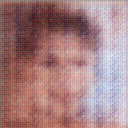
\includegraphics[width=150px]{500_fake_images/samples_5_274.png}%
\caption{A Close Up Of A Person Wearing A Tie}%
\end{figure}

%
\end{document}